\documentclass[pdftex,12pt,a4paper]{article}

\usepackage{graphicx}  
\usepackage[margin=2.5cm]{geometry}
\usepackage{breakcites}
\usepackage{indentfirst}
\usepackage{pgfgantt}
\usepackage{pdflscape}
\usepackage{float}
\usepackage{epsfig}
\usepackage{epstopdf}
\usepackage[cmex10]{amsmath}
\usepackage{stfloats}
\usepackage{multirow}
\usepackage{fixltx2e}

\renewcommand{\refname}{REFERENCES}
\linespread{1.3}

\usepackage{mathtools}
%\newcommand{\HRule}{\rule{\linewidth}{0.5mm}}
\thispagestyle{empty}
\begin{document}
	\begin{titlepage}
		\begin{center}
			\textbf{}\\
			\textbf{\Large{ISTANBUL TECHNICAL UNIVERSITY}}\\
			\vspace{0.5cm}
			\textbf{\Large{COMPUTER ENGINEERING DEPARTMENT}}\\
			\vspace{4cm}
			\textbf{\Large{BLG 222E\\ COMPUTER ORGANIZATION\\ PROJECT 2 REPORT}}\\
			\vspace{4cm}
			\begin{table}[ht]
				\centering
				\Large{
					\begin{tabular}{lcl}
						\textbf{CRN}  & : & 21335 \\
						\textbf{LECTURER}  & : & Prof. Dr. Deniz Turgay Altılar \\
				\end{tabular}}
			\end{table}
			\vspace{1cm}
			\textbf{\Large{GROUP MEMBERS:}}\\
			\begin{table}[ht]
				\centering
				\Large{
					\begin{tabular}{rcl}
						1500220079  & : & AHMET ENES ÇİĞDEM \\
				\end{tabular}}
			\end{table}
			\vspace{2.8cm}
			\textbf{\Large{SPRING 2024}}
			
		\end{center}
		
	\end{titlepage}
	
	\thispagestyle{empty}
	\addtocontents{toc}{\contentsline {section}{\numberline {}FRONT COVER}{}}
	\addtocontents{toc}{\contentsline {section}{\numberline {}CONTENTS}{}}
	\setcounter{tocdepth}{4}
	\tableofcontents
	\clearpage
	
	\setcounter{page}{1}
	
	\section{INTRODUCTION}
	
	In this raport I will basicly explain a CPU system with Arithmetic Logic Unit System and Contro Unit. ALU System is already impelmented befor. This raport will be mostly about Control Unit and CPU System.  
	
	\section{MATERIALS AND METHODS}
	Implementation of this project is made by using given instruction table. This table executed by an ALU System which is made before the Control Unit. Control Unit designed to control the inputs of ALU System and manipulate the RTL system according to corresponding operations in Figure 2.
	ALU System shown in Figure 1:
	
	\subsection{Programming Language}
	This project is implemented by using Verilog HDL. The operations and the ALU system is shown in figures 
	\begin{figure}[H]
		\centering
		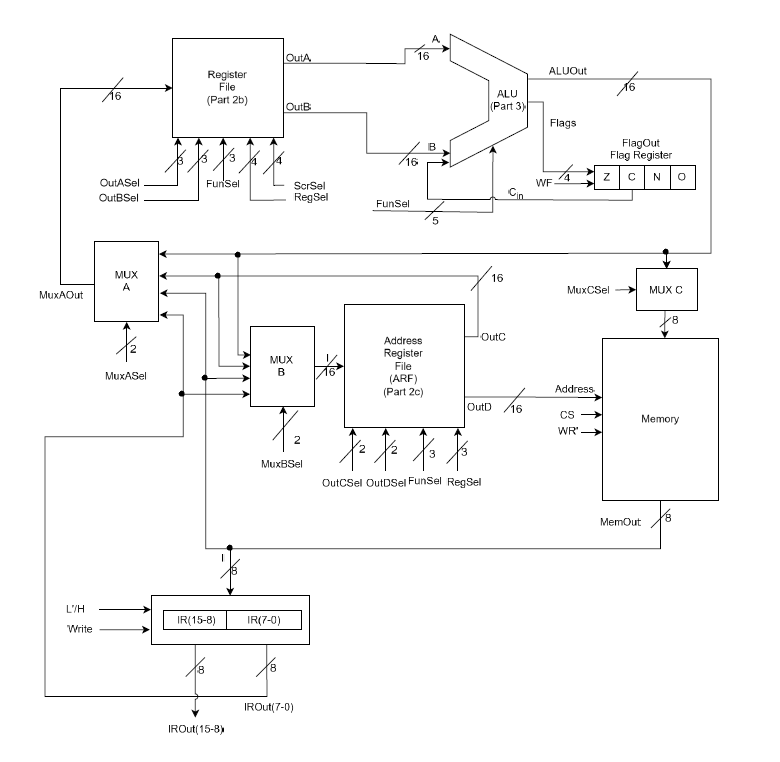
\includegraphics[width=0.8\textwidth]{ALUSystem.png}
		\caption{ALU System}
		\label{fig:ALU System}
	\end{figure}
	\begin{figure}[H]
		\centering
		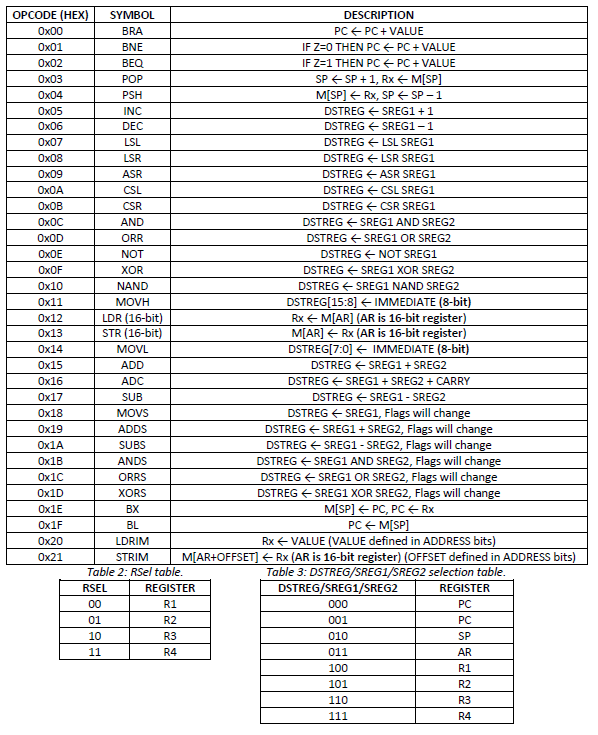
\includegraphics[width=1.0\textwidth]{OPCODES.png}
		\caption{Operation Codes}
		\label{fig:Operation Codes}
	\end{figure}
	\newpage
	\subsection{Implementation}
	The general implementation of this project is made by using clock cycle. No matter what type operation is being executed, the system goes throughout T based time loop and each operation change the inputs of ALU System based on their op code and other bits of instruction. When instruction is idetifed the inputs of the system will be arranged according to our operation.\par
	\textbf{Fetch and Decode}\par
	First I want to explain the fetch and decode steps of this RTL. In the fetch side our IR is 16 bits but our Memory words are 8 bits long so we need to first put instructions to IR in 2 clock cycle. T\textsubscript{0} and T\textsubscript{1}.\par
	These instructions are read from memory whit program counter adress after the fetch we will have new adress if we need for operation.\par
	\textbf{T}\textsubscript{0}: IR[7:0] \xleftarrow{}M[PC], PC \xleftarrow{} PC + 1\par
	\textbf{T}\textsubscript{1}: IR[15:8] \xleftarrow{}M[PC], PC \xleftarrow{} PC + 1\par
	After the fetch operation, we need to determine DSTREG, SREG1 and SREG2 for register referance instructions and RSEL for address referance then put the address to AR if we need.\par
	\textbf{T}\textsubscript{2}: AR \xleftarrow{} IR[7:0]\par
	And we need to identfy our input acoording to DSTREG, SREG1, SREG2 and RSEL. DSTREG is the register that will be written something so it must manipulate the RegSel of our ARF or RF and SREGs must determine the OutSel inputs. The basic match code is in the figure.
	When we need them, thanks to this code, we will just write these to corresponding inputs. 
	\begin{figure}[H]
		\centering
		\includegraphics[width=0.5\textwidth]{match-regs.png}
		\caption{Matching for registers}
		\label{fig:Operation Codes}
	\end{figure}\par 
	Then we need to identify what is our operation. I have 33 operations on this project but there could be more ,so for just to make it more flexible to more operation, I will make a 64 bits D register that will make the cooresponding binary cod 1 and others 0 according to operation code.\newpage
	\textbf{D}[IR[15:10]] = 1.\\
	This register show me what is the operation is according to op code written in IR[15:10]. All of these operations happen in clock T\textsubscript{2}.\par
	All of these for fetch and decode, now lets begin to execute operations. \par
	\textbf{Execution of some operations} \par
	
	\textbf{BRA}:\par
	T\textsubscript{3}: S1 \xleftarrow{} PC\par
	T\textsubscript{4}: S2 \xleftarrow{} IR[7:0]\par
	T\textsubscript{5}: PC \xleftarrow{} S1 + S2\par
	BNE and BNQ same as BRA just depend on Z as well.\par
	\textbf{POP}:\par
	T\textsubscript{3}: M[SP] \xleftarrow{} Rx[7:0], SP \xleftarrow{} SP + 1\par
	T\textsubscript{4}: M[SP] \xleftarrow{} Rx[7:0], SP \xleftarrow{} SP + 1\par
	\textbf{INC}:\par
	T\textsubscript{3}: DSTREG \xleftarrow{} SREG1\par
	T\textsubscript{4}: DSTREG \xleftarrow{} DSTREG + 1\par
	In DEC just the register functin is changed.\par
	\textbf{LSL}:\par
	In LSL for the RF is source and destination it can be handled in just one clock cycle.\par
	T\textsubscript{3}: DSTREG \xleftarrow{} LSL SREG1\par
	The output of ALU is equal to LSL SREG1 so we just write it DSTREG.\par
	LSR, ASR, CSL, CSR is same as this operation just ALU Funsel will be changed for each opeartin.\par
	\textbf{AND}:\par
	Same as the LSR if it's just for RF the result is directly writable to DSTREG.\par
	T\textsubscript{3}: DSTREG \xleftarrow{} SREG1 \land SREG2\par
	Operations OR NOT XOR NAND ADD SUB ADDS SUBS ANDS ORRS XORS is same as operation just ALU Funsel will be changed for corresponding operation.\par
	\textbf{STRIM}:\par
	T\textsubscript{3}: S1 \xleftarrow{} AR\par
	T\textsubscript{4}: S2 \xleftarrow{} IR[7:0]\par
	T\textsubscript{3}: AR \xleftarrow{} S1 + S2\par
	T\textsubscript{3}: M[AR] \xleftarrow{} Rx[7:0], AR \xleftarrow{} AR + 1\par
	T\textsubscript{3}: M[AR] \xleftarrow{} Rx[15:8]\par
	Example output for STRIM in the results section.
	
	
	
	
	
	
	
	
	\section{RESULTS }
	Example results for some operations:\par
	\textbf{BRA 0x28}
	\begin{figure}[H]
		\centering
		\includegraphics[width=0.8\textwidth]{ınc1.png}
		\caption{BRA 1}
		\label{fig:Operation Codes}
	\end{figure}\par 
	\begin{figure}[H]
		\centering
		\includegraphics[width=0.8\textwidth]{ınc2.png}
		\caption{BRA 2}
		\label{fig:Operation Codes}
	\end{figure}\par 
	\begin{figure}[H]
		\centering
		\includegraphics[width=0.8\textwidth]{ınc3.png}
		\caption{BRA 3}
		\label{fig:Operation Codes}
	\end{figure}\par 
	\begin{figure}[H]
		\centering
		\includegraphics[width=0.8\textwidth]{ınc4.png}
		\caption{BRA 4}
		\label{fig:Operation Codes}
	\end{figure}\par 
	
	
	\textbf{INC R1, R2}\par
	\begin{figure}[H]
		\centering
		\includegraphics[width=0.8\textwidth]{arttır1.png}
		\caption{INC 1}
		\label{fig:Operation Codes}
	\end{figure}\par 
	\begin{figure}[H]
		\centering
		\includegraphics[width=0.8\textwidth]{arttır2.png}
		\caption{INC 2}
		\label{fig:Operation Codes}
	\end{figure}\par 
	\begin{figure}[H]
		\centering
		\includegraphics[width=0.8\textwidth]{arttır3.png}
		\caption{INC 3}
		\label{fig:Operation Codes}
	\end{figure}\newpage
	\textbf{STRIM, R1, 0x10}\par
	\begin{figure}[H]
		\centering
		\includegraphics[width=0.8\textwidth]{strım1.png}
		\caption{STRIM 1}
		\label{fig:Operation Codes}
	\end{figure}\par 
	\begin{figure}[H]
		\centering
		\includegraphics[width=0.8\textwidth]{strım2.png}
		\caption{STRIM 2}
		\label{fig:Operation Codes}
	\end{figure}\par 
	\begin{figure}[H]
		\centering
		\includegraphics[width=0.8\textwidth]{strım3.png}
		\caption{STRIM 3}
		\label{fig:Operation Codes}
	\end{figure}\par 
	\begin{figure}[H]
		\centering
		\includegraphics[width=0.8\textwidth]{strım4.png}
		\caption{STRIM 4}
		\label{fig:Operation Codes}
	\end{figure}\par 
	\begin{figure}[H]
		\centering
		\includegraphics[width=0.8\textwidth]{strım5.png}
		\caption{STRIM 5}
		\label{fig:Operation Codes}
	\end{figure}\par 
	
	\section{DISCUSSION}
	In our CPU development, combining the ALU with the CU was a milestone. However, we faced a hurdle fetching ALU inputs through RTL with the CU. Coordinating CU control logic with ALU data processing proved challenging. Despite meticulous planning, routing and synchronizing inputs proved tricky due to data flow complexities and timing issues. Overcoming these challenges demanded a deeper understanding of hardware interactions. Through iterative refinement and experimentation, we navigated these hurdles, showcasing our team's adaptability and commitment to innovation.
	
	
	
	
	\section{CONCLUSION}
	
	In conclusion, our journey to integrate the ALU with the CU in our CPU architecture was filled with challenges and triumphs. Despite significant hurdles in fetching inputs for the ALU through RTL, our team's perseverance and collaboration prevailed. Through theoretical understanding, practical experimentation, and iterative refinement, we successfully addressed complexities in data routing and synchronization. This underscores our resilience and commitment to innovation, positioning us at the forefront of CPU architecture advancement. Moving forward, we are dedicated to pushing the boundaries of hardware design, driving continued progress and innovation in computing.
	
	
	\newpage
	\addcontentsline{toc}{section}{\numberline {}REFERENCES}
	
	\bibliographystyle{unsrt}
	\bibliography{reference}
	
\end{document}

